\documentclass[11pt]{amsart}

\usepackage{amsmath,amssymb,amsthm,mathtools}
\usepackage{stmaryrd}
\usepackage{array}
\usepackage[T1]{fontenc}
\usepackage[expansion=false]{microtype}
\usepackage{tikz}
\usetikzlibrary{arrows.meta,positioning}
\usepackage[colorlinks=true,linkcolor=blue!55!black,citecolor=blue!55!black]{hyperref}
\usepackage{enumitem}

% ---- theorem environments ----
\theoremstyle{plain}
\newtheorem{theorem}{Theorem}[section]
\newtheorem{proposition}[theorem]{Proposition}
\newtheorem{lemma}[theorem]{Lemma}
\newtheorem{corollary}[theorem]{Corollary}
\theoremstyle{definition}
\newtheorem{definition}[theorem]{Definition}
\newtheorem{example}[theorem]{Example}
\newtheorem{remark}[theorem]{Remark}

% ---- notation ----
\renewcommand{\Vec}{\mathsf{Vec}}
\newcommand{\Set}{\mathsf{Set}}
\newcommand{\Cat}{\mathsf{Cat}}
\newcommand{\Cont}{\mathsf{Cont}}
\newcommand{\LinCont}{\mathsf{LinCont}}
\newcommand{\Fam}{\mathsf{Fam}}
\newcommand{\Mon}{\mathsf{Mon}}
\newcommand{\Comon}{\mathsf{Comon}}
\newcommand{\Alg}{\mathsf{Alg}}
\newcommand{\Mat}{\mathsf{Mat}}
\newcommand{\VCat}{\Vec\text{-}\mathsf{Cat}}
\newcommand{\op}{\mathrm{op}}
\newcommand{\Nat}{\mathrm{Nat}}
\newcommand{\End}{\mathrm{End}}
\newcommand{\id}{\mathrm{id}}
\newcommand{\Id}{\mathrm{Id}}
\newcommand{\ext}[1]{\llbracket #1 \rrbracket}
\newcommand{\pos}{P}
\newcommand{\fld}{\Bbbk}
\newcommand{\bul}{{-}}
\newcommand{\iso}{\cong}
\DeclareMathOperator{\dcoprod}{\textstyle\coprod}

\emergencystretch=2.5em  % absorb unbreakable inline-math compounds in prose

\title[Containers over $\Vec$]{Containers over $\Vec$:\\ the biproduct collapse and the extensivity crux}
\author{MacBeth}
\date{18 August 2026 (rev.\ 21 August 2026) --- internal expository note}

\begin{document}

\begin{abstract}
We work out how much of the theory of containers survives the base change
$\Set \rightsquigarrow \Vec$. A \emph{linear container} is an object
$(S,(P_s))$ of $\Fam(\Vec^\op)$ --- a set of shapes, each carrying a
vector space of positions --- and its extension is the endofunctor
$\ext{S,P}\,W = \bigoplus_{s} \Vec(P_s, W)$ on $\Vec$. The whole story is
governed by a single fact: $\Set$ is extensive and $\Vec$ is not. In $\Set$
the coproduct is a disjoint union, and this is exactly what lets one read the
shape set off the functor and makes the extension functor fully faithful. In
$\Vec$ the coproduct is a biproduct, and the same two properties fail
\emph{together}: shapes become invisible (a finite linear container is
$\Id^{\,N}$, determined by one number $N$), and the extension functor stops
being full (natural transformations may mix shapes; container morphisms may
not). The gap is the single inclusion $\dcoprod \subsetneq \bigoplus$. The same failure
demotes the comonoid theory --- the $\lhd$-comonoids of $\Fam(\Vec^\op)$ are only
\emph{families of $\fld$-algebras}, not algebroids --- but here we can say exactly
what went wrong and fix it: the correct home for a linear directed container is the
matrix bicategory $\Mat(\Vec)$, one hom-space per ordered pair of objects, whose
comonoids \emph{are} algebroids (B\'enabou), and the single-index theory is its
diagonal degeneration. The repair is to move the coproduct from the shape index to
the composition index. Read for applications, the same biproduct is a feature:
modelling a prompt as a one-shape linear container, ``handle either prompt $A$ or $B$''
is their coproduct, whose reply-space is the biproduct $A\oplus B$ --- so ``answer
either'' is the same object as ``ready for both''. This is
an orientation document for the grant's ``containers over other bases''
front; the objects here are the additive corner of the strict polynomial
functors --- equivalently the degree-one slice of the analytic (Schur functor)
lifting of containers to $\Vec$, where the Young-diagram classification
degenerates to the single number $N$ --- and we are scrupulous throughout about
what that literature owns and what the container framing adds.
\end{abstract}

\maketitle

\tableofcontents

\section{The question, and the one-line answer}

The reader knows the $\Set$ container story. A \emph{container} is a pair
$(S,P)$ with $S$ a set of \emph{shapes} and $P\colon S \to \Set$ a family of
\emph{position sets}; its extension is the endofunctor
\[
  \ext{S,P}\,X \;=\; \sum_{s\in S} \Set(P_s, X) \;=\; \sum_{s\in S} X^{P_s}
  \qquad (\Set \to \Set).
\]
Two facts make this theory rigid and useful. First, the shape set is
\emph{readable off the functor}: $\ext{S,P}(1) = \sum_s 1^{P_s} = S$, so
evaluation at the terminal object returns the shapes. Second, the extension
$\ext{\bul}\colon \Fam(\Set^\op) \to [\Set,\Set]$ is \emph{fully faithful},
with essential image the polynomial (familially representable) functors; the
data $(S,P)$ can be reconstructed from $F$. Together these say: containers
\emph{are} their extensions, and the extensions wear their combinatorics on
their sleeve.

Neil's steer opens a new front: keep the container idea but change the base,
so that the \emph{answer space is a vector space}. Fix a field $\fld$ and let the
positions be $\fld$-vector spaces and the extension land in $\Vec$. Concretely
we study the single functor
\[
  \ext{\bul}\colon \Fam(\Vec^\op) \longrightarrow [\Vec,\Vec],
  \qquad
  \ext{S,P}\,W \;=\; \bigoplus_{s\in S} \Vec(P_s, W),
\]
and ask the base-change question: \emph{which parts of the $\Set$ theory carry
over, and which break?}

\paragraph{The one-line answer.}
Everything is controlled by one difference between the bases:
\begin{center}\itshape
$\Set$ is extensive --- its coproduct is disjoint union --- and $\Vec$ is not
--- its coproduct is a biproduct.
\end{center}
The two rigidity facts above both rest on extensivity, and so both fail, and
they fail as \emph{one} phenomenon. Precisely:
\begin{enumerate}[label=(\alph*)]
\item \textbf{Shapes become invisible (objects).} The terminal object of
  $\Vec$ is the \emph{zero} object, so $\ext{S,P}(0)=0$: there is no ``$F(1)=S$''.
  Worse, for finite data $\ext{S,P} \iso \Id^{\,N}$ with $N=\sum_s \dim P_s$,
  so the functor remembers only the total dimension $N$ --- not the shapes, not
  even the partition of $N$ into shapes (Theorem~\ref{thm:collapse}).
\item \textbf{The extension stops being full (morphisms).} Natural
  transformations between extensions are indexed by the \emph{biproduct}
  $\bigoplus_t$, while container morphisms are indexed by the \emph{disjoint
  union} $\dcoprod_t$; the comparison is the inclusion
  $\dcoprod_t \hookrightarrow \bigoplus_t$, which misses every transformation
  that mixes two shapes (Theorem~\ref{thm:crux}).
\end{enumerate}
Both bullets are the single inclusion $\dcoprod \subsetneq \bigoplus$: in
$\Set$ these two coproducts coincide (extensivity), in $\Vec$ they do not.
That is the whole paper.

\paragraph{What is new, and what is not.}
The \emph{objects} here --- functors $W \mapsto \bigoplus_s \Vec(P_s,W)$ ---
are the additive (degree-one) corner of the strict polynomial functors of
Friedlander--Suslin, a highly developed theory; the analytic/Day side is the
theory of vector species and twisted commutative algebras; ``coproduct of
representables'' and its extensivity hypothesis belong to Diers' familial
representability; ``algebroid'' is Mitchell's. None of these objects is ours.
What the container framing \emph{adds} is the assembly: it introduces a
\emph{shape index} on top of these functors and then discovers, through the
computation of this note, that the shape index is not an invariant of the
functor --- and that its collapse (on objects) and the failure of fullness (on
morphisms) are the same event, the failure of extensivity. See
\S\ref{sec:neighbours} for the honest ledger.

\paragraph{Roadmap.}
\S\ref{sec:vecstructure} is a short recap of the base $\Vec$ itself --- what it has
(a zero object, biproducts, self-enrichment) and what it lacks that $\Set$ has
(extensivity above all) --- for the reader fluent in categories but new to the linear
instance. \S\ref{sec:defs} gives the definitions ($\Set$ and $\Vec$ side by side).
\S\ref{sec:lemmas} proves the three-lemma toolbox (a linear co-Yoneda lemma;
$h_P = \Vec(P,\bul)$ is additive and fully faithful; finite positions
distribute over $\bigoplus$). \S\ref{sec:collapse} is the biproduct collapse.
\S\ref{sec:crux} is the hom formula and the extensivity crux. \S\ref{sec:comp}
computes composition and probes comonoids (the algebroid guess, honestly
assessed). \S\ref{sec:algebroid} then resolves it: the correct home for a linear
directed container is the matrix bicategory $\Mat(\Vec)$, whose (co)monoids are
genuine algebroids, and the single-index theory is exactly its diagonal
degeneration. \S\ref{sec:eitherprompt} is the application face: handling either of two
prompts is the coproduct of their linear containers, and the biproduct collapse makes
``answer either'' the same object as ``ready for both''. \S\ref{sec:table} is the
carry-over table. \S\ref{sec:schur} sets our
objects against the analytic (Schur functor) lifting and locates them as its
degree-one corner. \S\ref{sec:neighbours} is the prior-art ledger, and
\S\ref{sec:open} the open questions.

\section{The structure of $\Vec$, for the container-minded}\label{sec:vecstructure}

Before the definitions, a short recap of the base itself. The reader here is fluent
in categories but may simply not have worked with the linear-algebra instance; the
whole note turns on a handful of structural facts about $\Vec$, and it is worth
having them in one place, side by side with $\Set$. Nothing in this section is
proved --- each fact is standard, and each is a signpost to the section where it does
real work.

\paragraph{What $\Vec$ has.}
\begin{description}[leftmargin=1.4em,style=nextline]
\item[A zero object.] $\Vec$ is \emph{pointed}: the space $0$ is at once terminal and
  initial. There is a unique map $V\to 0$ and a unique map $0\to V$, and they are the
  same object. This is the first thing that breaks the $\Set$ intuition, where
  terminal ($1$) and initial ($\varnothing$) are wildly different sets.
\item[Finite biproducts.] For finitely many spaces the coproduct and the product
  \emph{coincide}: $V_1\oplus\dots\oplus V_n$ carries both the injections
  $V_i\hookrightarrow\bigoplus$ (making it a coproduct) and the projections
  $\bigoplus\twoheadrightarrow V_i$ (making it a product), compatibly. This shared
  object is the \emph{biproduct}. It is the structural heart of the note: every
  collapse below is this one coincidence, viewed through a different lens, and
  \S\ref{sec:eitherprompt} reads it as a \emph{feature}.
\item[Kernels and cokernels.] $\Vec$ is \emph{abelian}: every map has a kernel and a
  cokernel, and every mono/epi is normal. Idempotents split; the endomorphism ring of
  a functor governs its decomposition into indecomposables
  (Krull--Schmidt--Azumaya, used in Theorem~\ref{thm:collapse}).
\item[Self-enrichment.] $\Vec$ is enriched over itself: each hom $\Vec(V,W)$ is again
  a \emph{vector space}, and composition is bilinear. This is what makes ``linear
  container'' more than a slogan --- the extension functor is a $\Vec$-functor, and
  the linear co-Yoneda lemma (Lemma~\ref{lem:coyoneda}), the engine of every
  computation below, is exactly the enriched Yoneda lemma read in $\Vec$.
\end{description}

\paragraph{What $\Vec$ lacks that $\Set$ has.}
\begin{description}[leftmargin=1.4em,style=nextline]
\item[Extensivity.] This is the one that matters. $\Set$ is \emph{extensive}: its
  coproduct is a genuine disjoint union, and a map into $A\sqcup B$ is a
  \emph{partition} of the domain into the part landing in $A$ and the part landing in
  $B$ (Carboni--Lack--Walters). $\Vec$ is \emph{not} extensive: its finite coproduct
  is the biproduct, and a map into $A\oplus B$ is a \emph{pair} of maps (into $A$ and
  into $B$) that may both be nonzero. The comparison is the strict inclusion
  \[
    \dcoprod\ \subsetneq\ \bigoplus,
  \]
  and every ``fails'' in this note is one avatar of it
  (Theorems~\ref{thm:collapse},~\ref{thm:crux}).
\item[Disjoint, complemented injections.] In $\Set$ the coproduct injections are
  disjoint ($A\cap B=\varnothing$ inside $A\sqcup B$) and each summand is
  complemented. In $\Vec$ the injections $A,B\hookrightarrow A\oplus B$ overlap in
  every vector $a+b$ with $a,b\neq0$; there is no ``which summand did this element
  come from?''. That missing partition is precisely the information a shape function
  records and a biproduct destroys.
\item[A subobject classifier.] $\Set$ is a topos; $\Vec$ is not. There is no
  $\Omega$, so ``subset'' is not representable and the topos-theoretic tools that
  support the $\Set$ container calculus are unavailable. (We do not use them; the
  note leans on additivity and Krull--Schmidt instead.)
\item[A shape-detecting terminal object.] In $\Set$ the terminal object $1$ is a
  \emph{separator} that sees shapes: $\ext{S,P}(1)=S$. In $\Vec$ the terminal object
  is $0$, and $\ext{S,P}(0)=0$ sees nothing. The slogan ``shapes $=$ points of
  $F(1)$'' is a fact about $\Set$, not about containers, and it does not survive the
  base change (\S\ref{sec:collapse}).
\end{description}

\paragraph{The punchline of the recap.}
Read the two lists against each other and a single line does all the work. Everything
$\Vec$ \emph{has} that we use --- biproducts, self-enrichment, Krull--Schmidt --- and
the one thing it \emph{lacks} that we miss --- extensivity --- are two faces of the
same coin: the finite coproduct is a biproduct. Where $\Set$ keeps its summands
disjoint, $\Vec$ merges them, and $\dcoprod\subsetneq\bigoplus$ is the record of that
merge. The rest of the note is the systematic consequence of this one difference, and
\S\ref{sec:eitherprompt} shows that the ``merge'' is not only a liability for a
representation theorem but, read on the coproduct of two prompts, exactly the
structure an application wants.

\section{Definitions}\label{sec:defs}

Throughout, $\fld$ is a fixed field, $\Vec=\Vec_\fld$ is the category of all
$\fld$-vector spaces, $\Vec(V,W)$ is the hom \emph{vector space}, and
$[\Vec,\Vec]$ is the category of $\fld$-linear ($=$ additive) endofunctors and
natural transformations. Every functor $F\colon \Vec\to\Vec$ below is a
$\Vec$-functor: its action on homs $\Vec(V,W)\to\Vec(FV,FW)$ is $\fld$-linear.

\begin{definition}[linear container]\label{def:lincont}
A \emph{linear container} is an object of $\LinCont := \Fam(\Vec^\op)$: a pair
$(S,(P_s)_{s\in S})$ with $S$ a set (the \emph{shapes}) and each
$P_s\in\Vec$ (the \emph{position space} of shape $s$). A morphism
$(S,(P_s))\to(T,(Q_t))$ is a pair $(f,(\varphi_s))$ where $f\colon S\to T$ is a
function and, for each $s\in S$, $\varphi_s\colon Q_{f(s)}\to P_s$ is a linear
map --- contravariant on positions, exactly as for $\Set$ containers. Write
$n_s := \dim P_s$.
\end{definition}

Compare the $\Set$ definition: there $P_s$ is a \emph{set} and $\varphi_s\colon
Q_{f(s)}\to P_s$ a \emph{function}. Everything is the same except the base of
the position fibres, $\Set^\op \rightsquigarrow \Vec^\op$.

\begin{example}
$(\{*\},\,\fld^2)$ is the one-shape container whose single shape has a
two-dimensional position space. $(\{*_1,*_2\},\,(\fld,\fld))$ is the two-shape
container, each shape one-dimensional. These are \emph{different} objects of
$\Fam(\Vec^\op)$ (different shape sets). Watch them: they are the running
counterexample of the whole note.
\end{example}

\begin{definition}[extension]\label{def:ext}
The \emph{extension} of $(S,P)$ is the functor $\ext{S,P}\colon\Vec\to\Vec$,
\[
  \ext{S,P}\,W \;:=\; \bigoplus_{s\in S} \Vec(P_s, W).
\]
Choosing a basis of $P_s$ gives $\Vec(P_s,W)\iso W^{n_s}$ naturally in $W$, so
$\ext{S,P}\,W \iso \bigoplus_{s\in S} W^{\,n_s}$, a ``direct sum of powers''.
On a morphism $(f,(\varphi_s))$ the natural transformation acts by
$(g_s)_s \mapsto (g_{f(s)}\circ\varphi_s)_s$. This makes
$\ext{\bul}\colon\Fam(\Vec^\op)\to[\Vec,\Vec]$ a functor.
\end{definition}

\begin{definition}[corepresentable]\label{def:corep}
For $P\in\Vec$ write $h_P := \Vec(P,\bul)\colon\Vec\to\Vec$, the
\emph{corepresentable} at $P$. Then $\ext{S,P}=\bigoplus_{s\in S} h_{P_s}$, and
$h_\fld = \Vec(\fld,\bul)\iso\Id$.
\end{definition}

So a linear container's extension is a coproduct of corepresentables, and the
unit corepresentable is the identity functor. This is the analog of ``a $\Set$
container is a coproduct of representables $X^{P_s}$'', with $X^{P_s}=
\Set(P_s,X)$ the represented functor at the set $P_s$.

\paragraph{A non-example.}
The functor $W\mapsto W\otimes_\fld W$ (tensor square) is a $\Vec$-endofunctor
but is \emph{not} the extension of any linear container: it is homogeneous of
degree $2$ (it scales like $\lambda^2$ under $W\xrightarrow{\lambda} W$),
whereas every $\ext{S,P}$ is additive (degree $1$). Linear containers see only
the degree-one world; the higher-degree strict polynomial functors
(symmetric, exterior, tensor powers) live outside $\Fam(\Vec^\op)$. This is the
first hint that ``linear container'' means ``functor built from $\Id$ under
$\bigoplus$'' --- more precisely, as Remark~\ref{rem:cocont} sharpens, a
\emph{cocontinuous} $\Vec$-endofunctor with finite-dimensional value on $\fld$
--- which the collapse theorem will make exact.

\section{The three-lemma toolbox}\label{sec:lemmas}

Everything downstream is assembled from three short lemmas: a linear co-Yoneda
lemma (how maps out of a corepresentable are pinned down by one element), the
additivity and full faithfulness of $h$, and the fact that finite-dimensional
positions let hom commute with $\bigoplus$. Prove these once and the rest is
bookkeeping.

\begin{lemma}[linear co-Yoneda]\label{lem:coyoneda}
For any $\Vec$-functor $G\colon\Vec\to\Vec$ and any $P\in\Vec$ there is an
isomorphism of vector spaces $\Nat(h_P,G)\iso G(P)$, natural in $G$ and $P$. In
particular $\Nat(\Id,G)\iso G(\fld)$ and $\Nat(h_P,h_Q)\iso\Vec(Q,P)$.
\end{lemma}

\begin{proof}
Given $\alpha\colon h_P\Rightarrow G$, set $\xi:=\alpha_P(\id_P)\in G(P)$. For
any $\varphi\colon P\to W$, naturality of $\alpha$ along the postcomposition map
$\varphi_*\colon\Vec(P,P)\to\Vec(P,W)$ gives
\[
  \alpha_W(\varphi)=\alpha_W(\varphi_*\,\id_P)=G(\varphi)\bigl(\alpha_P\id_P\bigr)
  = G(\varphi)(\xi),
\]
so $\alpha$ is determined by $\xi$. Conversely, for $\xi\in G(P)$ define
$\alpha_W(\varphi):=G(\varphi)(\xi)$; this is linear in $\varphi$ because $G$ is
a $\Vec$-functor (so $\varphi\mapsto G(\varphi)$ is linear) followed by
evaluation at $\xi$, and natural in $W$ by functoriality of $G$. The two
constructions are mutually inverse and $\fld$-linear in $\xi$, so
$\Nat(h_P,G)\iso G(P)$. For $G=h_Q$, $G(P)=\Vec(Q,P)$.
\end{proof}

\begin{remark}
This is the enriched co-Yoneda lemma read in $\Vec$; the only wrinkle over the
ordinary Yoneda argument is that we need $\varphi\mapsto\alpha_W(\varphi)$ to be
\emph{linear}, which is exactly what ``$G$ is a $\Vec$-functor'' buys us.
\end{remark}

\begin{lemma}[$h$ is additive and fully faithful]\label{lem:h}
The assignment $h\colon\Vec^\op\to[\Vec,\Vec]$, $P\mapsto h_P$, is fully
faithful and sends finite biproducts to biproducts:
$h_{P\oplus Q}\iso h_P\oplus h_Q$. Consequently the only indecomposable
corepresentable is $h_\fld\iso\Id$, and $\End(\Id)=\fld$.
\end{lemma}

\begin{proof}
Full faithfulness is Lemma~\ref{lem:coyoneda} with $G=h_Q$:
$\Nat(h_P,h_Q)\iso\Vec(Q,P)=\Vec^\op(P,Q)$. Additivity:
$h_{P\oplus Q}(W)=\Vec(P\oplus Q,W)\iso\Vec(P,W)\times\Vec(Q,W)=(h_P\oplus
h_Q)(W)$, using that a finite product in $\Vec$ is a biproduct and that
biproducts in $[\Vec,\Vec]$ are computed pointwise; naturality is clear. Since
any $P$ with $\dim P\ge 2$ splits as $\fld\oplus(\cdots)$ and $h$ is additive,
$h_P$ decomposes unless $\dim P=1$; and $h_0=0$. So the unique indecomposable
corepresentable is $h_\fld$. Finally $\End(\Id)=\Nat(\Id,\Id)\iso\Id(\fld)=\fld$ by
Lemma~\ref{lem:coyoneda}.
\end{proof}

\begin{lemma}[finite positions distribute over $\bigoplus$]\label{lem:distribute}
If $\dim P<\infty$ then for any family $(V_t)_{t\in T}$,
$\Vec\bigl(P,\bigoplus_t V_t\bigr)\iso\bigoplus_t\Vec(P,V_t)$, naturally.
Equivalently, $h_P$ preserves coproducts iff $P$ is finite-dimensional.
\end{lemma}

\begin{proof}
Let $e_1,\dots,e_n$ be a basis of $P$. A linear map
$\varphi\colon P\to\bigoplus_t V_t$ is determined by the finite tuple
$(\varphi e_1,\dots,\varphi e_n)$, and each $\varphi e_i$ has finite support in
$T$; hence $\operatorname{im}\varphi$ lies in a finite subsum
$\bigoplus_{t\in F}V_t$. Therefore $\varphi$ lies in $\bigoplus_t\Vec(P,V_t)$
(the finitely supported families): this is the inclusion $\supseteq$; the
reverse inclusion is immediate. For $P$ infinite-dimensional the identity
$P\to P=\bigoplus_{i\in I}\fld$ has infinite support, so it lies in $\prod_i\fld$
but not $\bigoplus_i\fld$, and the isomorphism fails.
\end{proof}

The three lemmas already announce the theme. Lemma~\ref{lem:h} says the only
indecomposable brick is $\Id$; Lemma~\ref{lem:distribute} says that with finite
data the extension is a \emph{coproduct} of copies of $\Id$; and once a
coproduct of copies of $\Id$ over a \emph{finite} index becomes a biproduct,
the shapes are gone. That is the next section.

\section{Part 1 --- the biproduct collapse}\label{sec:collapse}

\subsection{Terminal recovery fails; the replacement}

The terminal object of $\Vec$ is the zero object $0$ (terminal $=$ initial in
an additive category). Hence
\[
  \ext{S,P}(0)=\bigoplus_{s\in S}\Vec(P_s,0)=\bigoplus_s 0 = 0.
\]

\begin{center}
\fbox{\parbox{0.92\linewidth}{\small
\textbf{Teachbox: always ask what the terminal object is.} The $\Set$ slogan
``$F(1)=S$'' is not a theorem about containers; it is a theorem about
$\Set$, whose terminal object $1$ is a \emph{separator} that detects shapes.
Change the base to $\Vec$, whose terminal object is $0$, and the slogan
evaporates: $\ext{S,P}(0)=0$ tells you nothing. The lesson generalises: when you
port a construction to a new base, the \emph{first} thing to recompute is the
terminal object and what it can see.}}
\end{center}

The natural evaluative replacement --- evaluate at the monoidal unit $\fld$
instead of at the terminal object --- fares only slightly better:
\[
  \ext{S,P}(\fld)=\bigoplus_s\Vec(P_s,\fld)=\bigoplus_s P_s^*,
  \qquad \dim = \sum_s n_s.
\]
This records the \emph{total} position dimension $N=\sum_s n_s$, and even that
only as a bare vector space --- with no partition into shapes. The honest
replacement for ``shapes $=$ points of $F(1)$'' is not evaluative but
\emph{homological}:
\begin{center}\itshape
shapes over $\Vec$ $=$ indecomposable direct summands of the functor $F$
\end{center}
--- and the next theorem measures how badly even that differs from the naive
shape set.

\subsection{Finite collapse}

\begin{theorem}[finite collapse]\label{thm:collapse}
Let $S$ be finite and every $n_s=\dim P_s$ finite, and set
$N:=\sum_{s\in S}n_s=\dim\bigl(\bigoplus_{s}P_s\bigr)$. Then there is a natural
isomorphism $\ext{S,P}\iso\Id^{\,N}$. Consequently:
\begin{enumerate}
\item $\ext{S,P}\iso\ext{S',P'}$ as functors \emph{iff} $N=N'$. A finite linear
  container is classified up to isomorphism of its extension by the single
  number $N$.
\item $\Id$ is indecomposable with $\End(\Id)=\fld$, and $\End(\Id^{\,N})=M_N(\fld)$
  is semiperfect, so by the Krull--Schmidt--Azumaya theorem the decomposition
  $\ext{S,P}\iso\Id^{\,\oplus N}$ into indecomposables is unique up to
  isomorphism and permutation. The recovered invariant is exactly the
  multiplicity $N$; the shape set $S$ and the partition $N=\sum_s n_s$ are
  \emph{not} recoverable.
\end{enumerate}
\end{theorem}

\begin{proof}
Choosing a basis of each $P_s$, $\Vec(P_s,W)\iso W^{n_s}$ naturally in $W$.
Since $S$ is finite,
\[
  \ext{S,P}\,W=\bigoplus_{s\in S}\Vec(P_s,W)\iso\bigoplus_{s\in S}W^{n_s}
  =W^{\,\sum_s n_s}=\Id^{\,N}(W),
\]
naturally in $W$; this is the isomorphism. Part (1): $\Id^{\,N}\iso\Id^{\,N'}$
iff $N=N'$ (evaluate at $\fld$). Part (2): $\Id$ is indecomposable because
$\End(\Id)=\fld$ has no idempotents $\neq 0,1$; $[\Vec,\Vec]$ is additive and
idempotent-complete (idempotents split pointwise, as $\Vec$ is), and
$\End(\Id^{\,N})=M_N(\fld)$ is Artinian hence semiperfect, so
Krull--Schmidt--Azumaya applies and gives uniqueness of the multiplicity.
\end{proof}

\begin{remark}[additive is not enough --- the hypothesis is \emph{cocontinuous}]\label{rem:cocont}
The collapse is a statement about \emph{cocontinuous} functors, not merely
additive ones, and the distinction is real. Additivity alone does not force
$\Id^{\,N}$: the corepresentable $h_P=\Vec(P,\bul)$ with $\dim P=\infty$ is
additive but a \emph{product} functor $\prod_I W$, not a coproduct of copies of
$\Id$ (Lemma~\ref{lem:distribute}); and $W\mapsto W^{**}$ is additive yet not of
the form $\Id^{\,N}$. The correct hypothesis is \emph{cocontinuity}
(preservation of coproducts). By the \emph{Eilenberg--Watts theorem}, a
$\Vec$-cocontinuous $\fld$-linear $F\colon\Vec\to\Vec$ is
$F\iso F(\fld)\otimes_\fld\bul\iso\Id^{\,\oplus\dim F(\fld)}$; so
$\dim F(\fld)=N<\infty$ gives $F\iso\Id^{\,N}$, with the only indecomposable
being $\Id$. A \emph{finite} linear container is cocontinuous --- this is
exactly Lemma~\ref{lem:distribute} (finite positions distribute over
$\bigoplus$) together with finiteness of $S$ --- which is why
Theorem~\ref{thm:collapse} applies. This is the intrinsic characterization made
sharp in Corollary~\ref{cor:recovery}, and it is the single clean use of
Eilenberg--Watts in this note.
\end{remark}

\begin{example}[the collapse in one picture]\label{ex:collapse}
Return to the running pair. Both
\[
  (\{*\},\,\fld^2)\quad\text{and}\quad(\{*_1,*_2\},\,(\fld,\fld))
\]
have extension $\Id^2$, i.e.\ $W\mapsto W^2$, though they have different shape
sets. Over $\Set$ the analogous containers $(\{*\},2)$ and
$(\{*_1,*_2\},(1,1))$ have \emph{distinct} extensions $X^2$ and $2\cdot X$, and
these are separated at $X=1$: $1^2=1\neq 2=2\cdot 1$. The collapse over $\Vec$
is \emph{precisely the loss of that separator} --- there is no object of $\Vec$
at which $W^2$ and $W\sqcup W$ come apart, because $\Vec$ has no separating
object that behaves like the one-point set.
\end{example}

\subsection{Where content survives}

The collapse used \emph{both} finiteness of $S$ (to turn $\bigoplus$ into a
finite biproduct) \emph{and} finite-dimensionality of the positions
(Lemma~\ref{lem:distribute}). Drop either and content returns.

\begin{description}
\item[Infinite $S$.] With all $P_s=\fld$, $\ext{S,P}=\bigoplus_{s\in S}\Id=
  \Id^{\,\oplus|S|}$. For infinite $S$ this is \emph{not} representable and
  $\bigoplus_s\Id\neq\prod_s\Id$: the functor is genuinely new. Still,
  Krull--Schmidt--Azumaya recovers only the cardinal $|S|$ (the number of $\Id$
  summands), not any finer shape structure.
\item[Infinite-dimensional positions.] By Lemma~\ref{lem:distribute}, $h_P$ for
  $\dim P=\infty$ does \emph{not} preserve coproducts:
  $h_P(W)=\Vec(P,W)\iso\prod_{i\in I}W$ is an \emph{infinite product} functor,
  not a coproduct of copies of $\Id$. Such $h_P$ are not built from $\Id$ under
  $\bigoplus$, and by Lemma~\ref{lem:h} distinct infinite-dimensional $P$ give
  non-isomorphic $h_P$. Here $P$ \emph{is} recovered from a single
  representable.
\item[The morphism layer.] Even where objects collapse, the category
  $\Fam(\Vec^\op)$ and the natural-transformation spaces between extensions do
  not. That is Part~2, and it is where the extensivity crux lives.
\end{description}

\section{Part 2 --- the hom formula and the extensivity crux}\label{sec:crux}

The $\Set$ representation theorem says $\ext{\bul}\colon\Fam(\Set^\op)\to
[\Set,\Set]$ is fully faithful, with essential image the polynomial functors,
and $(S,P)$ recovered from $F$ as $S=\pi_0(\mathrm{el}\,F)$ with positions the
generic elements. We isolate which half survives over $\Vec$ and locate the
failure in one symbol.

\begin{theorem}[hom formula]\label{thm:hom}
For linear containers $(S,P)$, $(T,Q)$,
\[
  \Nat\bigl(\ext{S,P},\ext{T,Q}\bigr)\;\iso\;
  \prod_{s\in S}\ \bigoplus_{t\in T}\ \Vec(Q_t,P_s).
\]
\end{theorem}

\begin{proof}
$\ext{S,P}=\bigoplus_s h_{P_s}$ is a coproduct, so
$\Nat(\bigoplus_s h_{P_s},G)\iso\prod_s\Nat(h_{P_s},G)\iso\prod_s G(P_s)$ by
Lemma~\ref{lem:coyoneda}. With $G=\ext{T,Q}$, $G(P_s)=\bigoplus_t\Vec(Q_t,P_s)$.
\end{proof}

\begin{theorem}[container-hom]\label{thm:conthom}
The morphisms of $\Fam(\Vec^\op)$ are
\[
  \Fam(\Vec^\op)\bigl((S,P),(T,Q)\bigr)\;\iso\;
  \prod_{s\in S}\Bigl(\ \dcoprod_{t\in T}\ \Vec(Q_t,P_s)\Bigr),
\]
where $\dcoprod$ is the coproduct in $\Set$ (disjoint union): a morphism
assigns to each $s$ a choice $t=f(s)$ together with a linear map in
$\Vec(Q_{f(s)},P_s)$.
\end{theorem}

\begin{proof}
Immediate from Definition~\ref{def:lincont}: a morphism is $f\colon S\to T$
plus, for each $s$, an element $\varphi_s\in\Vec(Q_{f(s)},P_s)$; packaging
$(f(s),\varphi_s)$ as an element of the disjoint union $\dcoprod_t\Vec(Q_t,P_s)$
and ranging over $s$ gives the product.
\end{proof}

Put the two formulas side by side. They are identical except for one symbol:
\[
  \underbrace{\prod_{s}\ \dcoprod_{t}\ \Vec(Q_t,P_s)}_{\text{container morphisms}}
  \qquad\longrightarrow\qquad
  \underbrace{\prod_{s}\ \bigoplus_{t}\ \Vec(Q_t,P_s)}_{\text{natural transformations}}
\]
The map between them is the extension functor on homs. It is, componentwise, the
comparison from the coproduct-in-$\Set$ to the coproduct-in-$\Vec$.

\begin{theorem}[the extensivity crux]\label{thm:crux}
The functor $\ext{\bul}$ induces, on each hom, the canonical map
\[
  \prod_s\ \dcoprod_t\ \Vec(Q_t,P_s)\;\longrightarrow\;
  \prod_s\ \bigoplus_t\ \Vec(Q_t,P_s),
\]
which is componentwise the inclusion of the disjoint union $\dcoprod_t$ into the
biproduct $\bigoplus_t$, sending a choice $(t,\varphi)$ to the element supported
at $t$. Therefore:
\begin{enumerate}
\item \textbf{Not full.} As soon as some shape $s\in S$ admits two shapes
  $t\neq t'\in T$ with $\Vec(Q_t,P_s)\neq 0\neq\Vec(Q_{t'},P_s)$, there are
  natural transformations $\ext{S,P}\Rightarrow\ext{T,Q}$ outside the image of
  $\ext{\bul}$ --- namely any whose $s$-component is a genuine linear
  combination $\varphi_t+\varphi_{t'}$ supported on two shapes. The cokernel of
  the inclusion measures exactly the cross-shape linear combinations that the
  biproduct permits and a shape function $f$ forbids.
\item \textbf{Extensivity is the whole story.} Over $\Set$ the same computation
  gives $\Nat(\ext{S,P},\ext{T,Q})\iso\prod_s\bigoplus_t\Set(Q_t,P_s)$, where now
  $\bigoplus_t$ is the coproduct in $\Set$ --- the disjoint union $\dcoprod_t$.
  Hence container-hom $=\Nat$ and $\ext{\bul}$ is fully faithful: the classical
  representation theorem. The single change under $\Set\rightsquigarrow\Vec$ is
  that the coproduct in the hom formula splits into two inequivalent notions,
  $\dcoprod_t\subsetneq\bigoplus_t$.
\end{enumerate}
\end{theorem}

\begin{proof}
The description of the induced map is the naturality of the
$\ext{\bul}$-action against Theorems~\ref{thm:hom}--\ref{thm:conthom}: a
container morphism $(f,(\varphi_s))$ produces the natural transformation whose
$s$-component is the composite through the single summand $t=f(s)$, i.e.\ the
element of $\bigoplus_t\Vec(Q_t,P_s)$ supported at $f(s)$. The map
$\dcoprod_t X_t\to\bigoplus_t X_t$ (choice $\mapsto$ supported element) is
injective away from zero and misses every element with support of size $\ge 2$;
taking $X_t=\Vec(Q_t,P_s)\neq 0$ for two values of $t$ exhibits a missed
element, proving (1). For (2): in $\Set$,
$\Nat(\ext{S,P},\ext{T,Q})\iso\prod_s\ext{T,Q}(P_s)=\prod_s\sum_t\Set(Q_t,P_s)$,
and $\sum_t=\dcoprod_t$, so this equals $\Fam(\Set^\op)((S,P),(T,Q))$; the
induced map is the identity and $\ext{\bul}$ is fully faithful. The sole
difference over $\Vec$ is $\bigoplus_t\neq\dcoprod_t$.
\end{proof}

\begin{center}
\begin{minipage}{0.45\linewidth}\centering
\begin{tikzpicture}[>=Stealth, node distance=6mm and 14mm, baseline=(a1.base)]
  \node (a1) {$s$};
  \node[right=of a1] (t1) {$t$};
  \node[below=5mm of t1] (t2) {$t'$};
  \draw[->, thick] (a1) -- node[above,sloped,font=\scriptsize]{$\varphi$} (t1);
\end{tikzpicture}\\[2pt]
{\small container morphism: \emph{one} branch, $\dcoprod_t$}
\end{minipage}%
\hfill
\begin{minipage}{0.45\linewidth}\centering
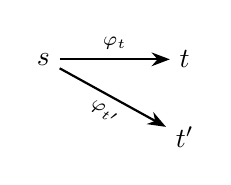
\begin{tikzpicture}[>=Stealth, node distance=6mm and 14mm, baseline=(a2.base)]
  \node (a2) {$s$};
  \node[right=of a2] (u1) {$t$};
  \node[below=5mm of u1] (u2) {$t'$};
  \draw[->, thick] (a2) -- node[above,sloped,font=\scriptsize]{$\varphi_t$} (u1);
  \draw[->, thick] (a2) -- node[below,sloped,font=\scriptsize]{$\varphi_{t'}$} (u2);
\end{tikzpicture}\\[2pt]
{\small natural transformation: a \emph{combination}, $\bigoplus_t$}
\end{minipage}
\end{center}
\noindent The left morphism lives in $\dcoprod_t$: it \emph{chooses} the
target shape $t=f(s)$. The right transformation lives in $\bigoplus_t$: it
sends $s$ into a \emph{linear combination} $\varphi_t+\varphi_{t'}$ of two
target shapes at once. In $\Set$ there is no such combination --- a function
must pick one branch --- which is exactly why the two hom sets coincide there.
In $\Vec$ the biproduct manufactures the combinations, and they are precisely
the transformations no container morphism can hit.

\begin{corollary}[finite recovery, sharp]\label{cor:recovery}
Restrict to finite containers with finite-dimensional positions. Then
$\ext{\bul}$ recovers from $\ext{S,P}$:
\begin{itemize}
\item the total position space $\bigoplus_{s\in S}P_s\in\Vec$ up to isomorphism
  (equivalently the number $N$), because $\bigoplus_s h_{P_s}\iso
  h_{\bigoplus_s P_s}$ (Lemma~\ref{lem:h}) and $h$ is fully faithful, so the
  extension determines $\bigoplus_s P_s$ exactly;
\item \emph{nothing} about the partition of $N$ into shapes.
\end{itemize}
Thus the honest representation statement over $\Vec$ is: $F$ is a finite linear
container $\iff F\iso\Id^{\,N}\iff F$ is $\Vec$-cocontinuous with $F(\fld)$
finite-dimensional; and the data $(S,P)$ is recovered only up to the biproduct
ambiguity --- a single object $\bigoplus_s P_s$ with no canonical shape
decomposition.
\end{corollary}

\begin{proof}
The two bullets are Theorem~\ref{thm:collapse} and Lemma~\ref{lem:h}. For the
intrinsic characterization: any $\Vec$-cocontinuous $F$ with $F(\fld)$
finite-dimensional is $F\iso F(\fld)\otimes\bul$ by the Eilenberg--Watts theorem,
and $\dim F(\fld)=N<\infty$ forces $F(\fld)\otimes\bul\iso\Id^{\,N}$; conversely
$\Id^{\,N}$ is manifestly of this form.
\end{proof}

\section{Part 3 --- composition and comonoids}\label{sec:comp}

Set containers compose by substitution, and the composite has shapes the
dependent sum $\dcoprod_{s\in S}T^{P_s}$ and positions the dependent pairs. Over
$\Vec$ the dependent sum flattens.

\begin{proposition}[composition of linear containers]\label{prop:comp}
For linear containers with finite-dimensional positions,
\[
  \ext{S,P}\circ\ext{T,Q}\;\iso\;\ext{\,S\times T,\ (P_s\otimes Q_t)_{(s,t)}\,},
\]
so on $\Fam(\Vec^\op)$ (finite-dimensional positions) composition is
$(S,P)\lhd(T,Q)=(S\times T,\ (P_s\otimes Q_t))$, with unit $I=(\{*\},\fld)$
(extension $\Id$).
\end{proposition}

\begin{proof}
We compute the composite on an object $W$:
\[
  \ext{S,P}\bigl(\ext{T,Q}\,W\bigr)
  =\bigoplus_s\Vec\Bigl(P_s,\ \textstyle\bigoplus_t\Vec(Q_t,W)\Bigr).
\]
Since $P_s$ is finite-dimensional, Lemma~\ref{lem:distribute} gives
$\Vec(P_s,\bigoplus_t\Vec(Q_t,W))\iso\bigoplus_t\Vec(P_s,\Vec(Q_t,W))$, and the
tensor--hom adjunction (with $P_s$ finite-dimensional) gives
$\Vec(P_s,\Vec(Q_t,W))\iso\Vec(P_s\otimes Q_t,W)$. Summing,
$\iso\bigoplus_{(s,t)}\Vec(P_s\otimes Q_t,W)$. The unit:
$(\{*\},\fld)\lhd(T,Q)=(\{*\}\times T,\ \fld\otimes Q_t)=(T,Q)$.
\end{proof}

\begin{remark}[why the dependent sum disappears]
Over $\Set$ the composite shapes are $\dcoprod_{s}T^{P_s}$: a composite shape is
a shape $s$ \emph{together with a function} $P_s\to T$ choosing a $T$-shape at
each position. Over $\Vec$, Lemma~\ref{lem:distribute} says a linear map
$P_s\to\bigoplus_t V_t$ is a \emph{sum of components}, not a \emph{choice of
branch}; the ``function $P_s\to T$'' has nowhere to live. So the dependency
$T^{P_s}$ collapses to the plain product $S\times T$, and the positions tensor.
Linearity flattens the dependent sum. This is the same $\dcoprod\subsetneq
\bigoplus$ phenomenon once more, now inside composition.
\end{remark}

\begin{proposition}[comonoids: the algebroid guess, honestly]\label{prop:comonoid}
A $\lhd$-comonoid $((S,P),\delta,\varepsilon)$ in
$(\Fam(\Vec^\op)_{\mathrm{fin}},\lhd,I)$ amounts to: the shape set $S$ (with its
unique $(\Set,\times)$-comonoid structure, the diagonal) together with, for each
$s\in S$, a $\fld$-algebra structure on $P_s$. In particular a one-shape
$\lhd$-comonoid $(\{*\},P)$ is exactly a $\fld$-algebra $P$.
\end{proposition}

\begin{proof}[Proof {\normalfont(sketch; full verification in the companion note)}]
The comultiplication $\delta\colon(S,P)\to(S,P)\lhd(S,P)=(S\times S,\
(P_a\otimes P_b))$ has shape component a function $S\to S\times S$; the counit
$\varepsilon\colon(S,P)\to I=(\{*\},\fld)$ has shape component $S\to\{*\}$.
Coassociativity and counitality of the shape components make $S$ a comonoid in
$(\Set,\times)$, which forces the diagonal $s\mapsto(s,s)$ (every set is
uniquely such a comonoid). With $a=b=s$, the position component of $\delta$ is a
family $\mu_s\colon P_s\otimes P_s\to P_s$, and of $\varepsilon$ a family
$\eta_s\colon\fld\to P_s$; coassociativity and counitality of $\delta$ become
associativity and the unit laws for $(\mu_s,\eta_s)$, i.e.\ a $\fld$-algebra on
each $P_s$. Distinct shapes never interact, because the diagonal cannot reach
the off-diagonal shape pairs $(a,b)$ with $a\neq b$.
\end{proof}

\begin{remark}[the crown target, honestly assessed]
The $\Set$ spine is $\text{poly-comonoid}\iso\text{small category}$
(directed containers $\iso$ categories); one hoped $\lhd$-comonoid over $\Vec
\iso\ \fld$-linear category (algebroid, in Mitchell's sense: a category enriched
in $\Vec$). Proposition~\ref{prop:comonoid} shows the finite-dimensional analog
is \emph{weaker}: a $\lhd$-comonoid yields only a \emph{family of $\fld$-algebras}
--- a ``diagonal'' algebroid with no morphisms between distinct objects ---
because the linear composition $\lhd$ of Proposition~\ref{prop:comp} has lost
the dependent-sum structure that, over $\Set$, lets a comonoid encode composable
arrows between different objects. The biproduct/linearity collapse strikes a
\emph{third} time, now degrading algebroids to algebra-families. Recovering a
full algebroid requires a genuinely different (lax, or bimodule) composition on
$\Fam(\Vec^\op)$; pinning that down is future work, and is the true $\Vec$
analog of the equivalence $\mathsf{DCont}\iso\Cat$ --- and \S\ref{sec:algebroid} identifies
that composition. \textbf{Status:} Proposition~\ref{prop:comonoid} is now
\emph{proved} (companion note \texttt{2026-08-19-vec-comonoids-algebras.md}): the
full statement is $\Comon_\lhd(\Fam(\Vec_{\mathrm{fd}}^\op))\iso\Fam(\Alg_\fld^\op)$,
with $S$ \emph{arbitrary} (finite $S$ not needed), the comonoid morphisms being
backward $\fld$-algebra homomorphisms, and an independent brute-force check over
$\fld=\mathbb F_2$ confirming that no off-diagonal comultiplication survives the
laws.
\end{remark}

\section{Part 4 --- the correct home: linear directed containers are
$\Vec$-matrices}\label{sec:algebroid}

Part 3 ended on an apparent defeat: the $\lhd$-comonoids of
$\Fam(\Vec^\op)$ are only \emph{families of algebras}, never a genuine algebroid,
and we flagged that recovering the full Mitchell notion ``requires a genuinely
different (lax, or bimodule) composition.'' This section identifies that
composition. The punchline is not a new theorem --- the mathematics here is
classical, due to B\'enabou and Mitchell --- but a \emph{diagnosis}: the naive
single-index theory was working with the wrong shape of data, and once the data is
corrected the algebroid reappears on the nose. The failure of Part 3 was not
$\Vec$'s fault; it was a modelling error, and pinpointing it turns the collapse
into a boundary we understand exactly.

\subsection{The reframe: shapes are objects, positions are homs}

Recall \emph{why} $\mathsf{DCont}\iso\Cat$ works over $\Set$
(Ahman--Uustalu). In a directed container the shapes are the \emph{objects} of the
category and the positions over a shape are the \emph{arrows out of that object};
composition of the container is composition of arrows. The dictionary is
\emph{shapes $=$ objects, positions $=$ arrows}.

A single-index linear container $(S,(P_s))$ cannot honour this dictionary, and now
we can see the reason sharply. It offers \emph{one} position space $P_s$
\emph{per shape} --- but a $\Vec$-enriched category (an algebroid) has a hom-space
$\hom(a,b)$ for each \emph{ordered pair} of objects. There is simply no room in the
index $s\in S$ to record ``an arrow \emph{from} $a$ \emph{to} $b$.'' In
$\Fam(\Vec^\op)$ the ``shapes'' behave as bare indices, not as objects with a homset
between each pair. So the correct linear analogue of a directed container is not a
family indexed by $S$ but a family indexed by $S\times S$.

\begin{definition}[$\Vec$-matrix / $\Vec$-graph]\label{def:vmat}
Fix a set $S$ (the \emph{objects}). A \emph{$\Vec$-matrix on $S$} is a family
$P=(P_{a,b})_{(a,b)\in S\times S}$ of finite-dimensional $\fld$-vector spaces: one
hom-space $P_{a,b}$ for each ordered pair. Write $\Mat_S(\Vec)$ for the category of
$\Vec$-matrices on $S$ and their entrywise linear maps. A $\Vec$-matrix is exactly a
$\Vec$-enriched graph on the vertex set $S$; equivalently it is a $1$-cell
$S\nrightarrow S$ of the bicategory $\Mat(\Vec)$ of sets, $\Vec$-matrices, and
matrix maps.
\end{definition}

This is the expected directed-container reindexing made linear: shapes have become
vertices/objects, and positions have become hom-objects \emph{between} vertices ---
positions are arrows, and an arrow needs a source \emph{and} a target.

\subsection{The lax composition is matrix product}

With the data corrected, the composition writes itself. Composing an arrow
$a\to b$ with an arrow $b\to c$ should yield an arrow $a\to c$, summed over all
possible intermediate objects $b$:

\begin{definition}[matrix composition]\label{def:matcomp}
For $\Vec$-matrices $P,Q$ on $S$, define $P\odot Q$ and the unit matrix $I$ by
\[
  (P\odot Q)_{a,c}\;:=\;\bigoplus_{b\in S} P_{a,b}\otimes Q_{b,c},
  \qquad
  I_{a,b}\;:=\;\begin{cases}\fld & a=b\\ 0 & a\neq b.\end{cases}
\]
This is $1$-cell composition in $\Mat(\Vec)$ restricted to a fixed object set:
matrix multiplication with $\otimes$ for entrywise product and $\bigoplus$ for
entrywise sum. It makes $(\Mat_S(\Vec),\odot,I)$ a monoidal category.
\end{definition}

Everything the collapse cost us is restored by the single symbol $\bigoplus_b$. Look
at where it sits: the sum ranges over the \emph{intermediate object} $b$, so it is
the \emph{composable-arrows sum} --- the linear reincarnation of the $\Set$
dependent sum $\dcoprod_{s} T^{P_s}$ that flattened in
Proposition~\ref{prop:comp}. Over $\Set$ a composite shape is ``a shape $s$
together with a choice of next shape at each position''; that dependency is exactly
a sum over the middle object, and the matrix product $\bigoplus_b P_{a,b}\otimes
Q_{b,c}$ is its faithful linear image. One honesty caveat, stated once and meant
precisely: this $\bigoplus_b$ is the \emph{right reincarnation} of the extensivity
coproduct whose absence ($\dcoprod\subsetneq\bigoplus$) drove the whole collapse ---
it is a $\bigoplus$ over the middle object, deployed \emph{where a categorical
composite needs it} --- but it is not literally the same coproduct as the one that
failed to be disjoint in Part~1. The point is structural, not an identity of
functors: putting the sum on the composition index, rather than on the shape index,
is what a category wants and what a plain family cannot express.

\subsection{Its (co)monoids are algebroids}

Now the classical fact, in the two variances we need.

\begin{proposition}[monoids in $\Mat_S(\Vec)$ are algebroids; B\'enabou]
\label{prop:algebroid-mon}
A monoid $(P,\mu,\eta)$ in $(\Mat_S(\Vec),\odot,I)$ is exactly a
$\fld$-linear category (algebroid, in Mitchell's sense) with object set $S$:
$\hom(a,b)=P_{a,b}$; the multiplication $\mu\colon P\odot P\to P$ is the family of
composition maps $\bigoplus_b P_{a,b}\otimes P_{b,c}\to P_{a,c}$; and the unit
$\eta\colon I\to P$ picks out the identity arrow $\fld\to P_{a,a}$ at each object.
Associativity of $\mu$ is associativity of composition; the unit laws are the
identity-arrow laws. Thus $\Mon(\Mat_S(\Vec),\odot,I)\iso\VCat_S$, the
$\fld$-linear categories with object set $S$.
\end{proposition}

This is B\'enabou's observation that a monad in a bicategory of matrices (or spans)
is an enriched category, specialised to $V=\Vec$ over the discrete base $S$; it is
the additive avatar of the poly-comonad $=$ category theorem
(Spivak; the $\Set$ spine $\mathsf{DCont}\iso\Cat$). The \emph{comonoid} version,
which is what a container theory delivers after the contravariant twist on
positions, follows by applying the fibrewise op.

\begin{proposition}[comonoids, via the fibrewise op]\label{prop:algebroid-comon}
Work with $\Vec$-matrices of finite-dimensional entries. The entrywise op
$P_{a,b}\rightsquigarrow P_{a,b}$ read in $\Vec^\op$ carries $\odot$ to $\odot$ (the
tensor is self-dual on finite-dimensional spaces and $\bigoplus$ is its own dual),
so a $\odot$-comonoid in $\Mat_S(\Vec^\op)$ is the same data as a $\odot$-monoid in
$\Mat_S(\Vec)$ --- both ops cancel. Hence
\[
  \Comon\bigl(\Mat_S(\Vec^\op),\odot,I\bigr)\;\iso\;\VCat_S
\]
as well: $\Vec$-enriched categories on object set $S$, now presented
comultiplicatively. The variance bookkeeping (which op lands where) is the
monad/comonad-in-$V$-$\Mat$ duality made explicit by Cruttwell--Shulman-style
enriched double-category arguments (arXiv:1704.00329).
\end{proposition}

So the crown target is reached: on the corrected data --- one hom-space per ordered
pair --- the linear $\lhd$-comonoids \emph{are} algebroids, exactly the $\Vec$
analogue of $\mathsf{DCont}\iso\Cat$. The open question 2 of Part 3 is answered in
the affirmative; the ``lax/bimodule composition'' it asked for is the matrix product
$\odot$.

\subsection{The strict single-index $\lhd$ is the diagonal degeneration}

Why, then, did Part 3 see only algebra-families? Because the single-index theory is
the \emph{diagonal} of the matrix theory --- the arrows-only-between-equal-objects
fragment.

\begin{proposition}[diagonal embedding]\label{prop:diagonal}
Send a single-index linear container $(S,(P_s))$ to the \emph{diagonal}
$\Vec$-matrix $\widehat P$ with $\widehat P_{a,b}=P_a$ if $a=b$ and $0$ otherwise.
Diagonal $\Vec$-matrices are closed under $\odot$:
\[
  (\widehat P\odot\widehat Q)_{a,c}
  =\bigoplus_{b} \widehat P_{a,b}\otimes\widehat Q_{b,c}
  =\begin{cases}P_a\otimes Q_a & a=c\\ 0 & a\neq c,\end{cases}
\]
because the only surviving summand is $b=a=c$. So $\odot$ restricts, on diagonal
matrices, to the \emph{pointwise} tensor $(P_a\otimes Q_a)_{a}$ with unit
$(\fld)_a$, and a $\odot$-(co)monoid supported on the diagonal is precisely a family
of $\fld$-(co)algebras --- a family of \emph{one-object} $\fld$-linear categories.
This is the content of Proposition~\ref{prop:comonoid}:
$\Comon_\lhd(\Fam(\Vec_{\mathrm{fd}}^\op))\iso\Fam(\Alg_\fld^\op)$ is the diagonal
fragment of $\Comon(\Mat_S(\Vec^\op),\odot,I)\iso\VCat_S$.
\end{proposition}

The reconciliation with Part 3 is worth stating carefully, because the two
compositions do differ off the diagonal. The strict single-index $\lhd$ of
Proposition~\ref{prop:comp} has shape set the \emph{full} product $S\times S$ and
fibre $P_a\otimes P_b$ over every pair $(a,b)$ --- it does \emph{not} agree with
$\odot$, whose composite is a $\bigoplus_b$ and lives back on $S$. What Part 3
proved is that the counit \emph{forces a single-index comonoid onto the diagonal}
(\S3 of the companion note: $\delta_{\mathrm{shape}}(s)=(s,s)$), so the
comultiplication only ever touches the fibres $P_s\otimes P_s\to P_s$ and the
off-diagonal fibres $P_a\otimes P_b$ ($a\neq b$) are structurally unreachable. In
other words the single-index comonoid theory \emph{cannot escape the diagonal}, and
on the diagonal it coincides with the genuine matrix theory of
Proposition~\ref{prop:diagonal}. The diagonalisation happens at two coupled levels
that are really one phenomenon:
\begin{enumerate}[label=(\roman*)]
\item \textbf{position-support diagonal} --- the embedding $\widehat P$ keeps only
  the $a=b$ hom-spaces (no arrows between distinct objects);
\item \textbf{shape-comultiplication diagonal} --- the counit forces
  $\delta_{\mathrm{shape}}=\Delta$, so the comonoid comultiplication lands only in
  the $(s,s)$ block.
\end{enumerate}
Both say the same thing: \emph{one object, no cross-object composition}, hence a
$\fld$-algebra rather than a $\fld$-linear category. This is why the crown looked
lost: the single-index framing had silently pre-restricted to the diagonal
sub-bicategory before the classification even began.

\subsection{The single obstruction, stated once}

We can now name the one fact that runs through all four parts of this note. Over
$\Set$ the coproduct is a disjoint union and the base is \emph{extensive}
(Carboni--Lack--Walters); over $\Vec$ the coproduct is a biproduct and extensivity
fails, $\dcoprod\subsetneq\bigoplus$. Every collapse in this note is that one
failure, viewed through a different structure:
\begin{itemize}
\item \textbf{objects} --- shapes become invisible, a finite linear container is
  $\Id^{\,N}$ (Theorem~\ref{thm:collapse});
\item \textbf{morphisms} --- the extension is not full, container morphisms are the
  $\dcoprod$-indexed fragment of the $\bigoplus$-indexed transformations
  (Theorem~\ref{thm:crux});
\item \textbf{comonoids} --- the $\lhd$-comonoids of $\Fam(\Vec^\op)$ are a family
  of algebras, the diagonal degeneration of an algebroid
  (Proposition~\ref{prop:comonoid}, \S\ref{sec:algebroid}).
\end{itemize}
And the algebroid \emph{reappears precisely when the matrix product restores the
sum over the intermediate object}: the $\bigoplus_b$ of Definition~\ref{def:matcomp}
is the composition-index coproduct that the single-index theory had no place to put.
The slogan of the whole note therefore sharpens from a diagnosis of failure into a
statement of exactly where the boundary lies:
\begin{center}\itshape
the naive linear $\mathsf{DCont}\iso\Cat$ fails because $\Vec$ is not extensive;
it is repaired by moving the coproduct from the shape index to the composition
index --- from families over $S$ to matrices over $S\times S$.
\end{center}

\begin{center}
\fbox{\parbox{0.92\linewidth}{\small
\textbf{Provenance note (internal), \S\ref{sec:algebroid}.} The mathematics of this
section is \emph{classical} and the section's only contribution is the
container-theoretic diagnosis (single-index $=$ diagonal degeneration; the matrix
$\bigoplus_b$ $=$ the composition-index coproduct; non-extensivity as the single
organising obstruction). \emph{Monoid in a matrix/span bicategory $=$ enriched
category} is B\'enabou (\emph{Introduction to bicategories}, LNM 47, 1967);
\emph{algebroid $=$ ring with several objects}, one object $=$ algebra, is Mitchell
(\emph{Rings with several objects}, Adv.\ Math.\ 8, 1972); the
monad/comonad-in-$V$-$\Mat$ variance guardrail (Proposition~\ref{prop:algebroid-comon})
is the enriched-duality-in-double-categories line, arXiv:1704.00329. The $\Set$
precedents lifted here are Ahman--Uustalu $\mathsf{DCont}\iso\Cat$ (arXiv:1604.01187)
and Spivak's polynomial-comonad $=$ category (arXiv:2202.00534, 2111.10968); the
non-extensivity of $\Vec$ is Carboni--Lack--Walters (JPAA 84, 1993). None of these is
deep-read into \texttt{sources.json} this cycle; before any external circulation,
direct-read D.\ Lin, \emph{Enriched Polynomial Functors}, to confirm it does not
already state this framing, and disambiguate from arXiv:1209.0940 / 1403.0833 (there
``linear'' means linear \emph{logic}, not $\Vec$-enrichment).}}
\end{center}

\section{Application: handling either prompt is the biproduct}\label{sec:eitherprompt}

The note so far has read the biproduct as a \emph{loss}: it erases shapes
(\S\ref{sec:collapse}) and breaks fullness (\S\ref{sec:crux}). This section turns the
same fact over and reads it as a \emph{gain}. The setting is the one that motivated the
front in the first place --- prompts and their responses --- and the payoff is a clean
categorical answer to a question Neil posed directly: \emph{prompt $A$ with reply-space
$A$, prompt $B$ with reply-space $B$; what vector space matches being able to handle
\textbf{either} prompt?} The answer is the coproduct of the two linear containers, and
the biproduct makes that answer coincide with ``be ready for \textbf{both}''.

\subsection{Prompts as one-shape linear containers}

Fix the modelling dictionary, which is Neil's. A response to a prompt is not a single
token but a \emph{distribution} --- a superposition of possible replies, carrying the
model's uncertainty --- so the space of responses is a vector space, and the basis in
which that space is expressed is what a learning system \emph{learns}. Responses $=$
uncertainty $=$ the basis of learning. A prompt is therefore packaged as a
\emph{one-shape linear container}: the single shape is the prompt, and its position
space is the reply space.

\begin{definition}[prompt container]\label{def:prompt}
A \emph{prompt with reply-space $A$} is the one-shape linear container
$\mathsf A:=(\{*\},A)\in\Fam(\Vec^\op)$, with extension the corepresentable
\[
  \ext{\mathsf A}\,W=\Vec(A,W)=h_A(W).
\]
A point of $\ext{\mathsf A}\,W$ is a linear map $A\to W$: a way of reading the reply
space into the ambient answer space $W$.
\end{definition}

\subsection{Either prompt is the coproduct; the coproduct is the biproduct}

``Handle either prompt $A$ or prompt $B$'' is a \emph{choice of prompt}, and choice is
coproduct. In $\Fam(\Vec^\op)$ the coproduct is the disjoint union of shape sets ---
the one place a set-level disjoint union survives untouched, because it indexes shapes,
not positions --- so it is the honest ``or''. The biproduct then does the rest.

\begin{proposition}[either-prompt $=$ biproduct]\label{prop:eitherprompt}
Let $\mathsf A=(\{*\},A)$ and $\mathsf B=(\{*\},B)$ be prompt containers. Their
coproduct in $\LinCont=\Fam(\Vec^\op)$ is the two-shape container
\[
  \mathsf A\sqcup\mathsf B=\bigl(\{*_A,*_B\},\,(A,B)\bigr),
\]
and its extension is the corepresentable at the biproduct $A\oplus B$:
\[
  \ext{\mathsf A\sqcup\mathsf B}
  \;=\;h_A\oplus h_B
  \;\iso\;h_{A\oplus B}
  \;=\;\ext{(\{*\},\,A\oplus B)}.
\]
Consequently, as functors, ``handle either prompt $A$ or prompt $B$'' is the
\emph{single} prompt whose reply-space is the biproduct $A\oplus B$.
\end{proposition}

\begin{proof}
The coproduct in $\Fam(\mathcal C)$ is disjoint union of indexing sets with the
position families juxtaposed, for any $\mathcal C$; hence
$\mathsf A\sqcup\mathsf B=(\{*_A,*_B\},(A,B))$. The extension functor sends this
coproduct to the pointwise biproduct,
$\ext{\mathsf A\sqcup\mathsf B}W=\Vec(A,W)\oplus\Vec(B,W)=(h_A\oplus h_B)(W)$,
directly from Definition~\ref{def:ext}. Finally $h_A\oplus h_B\iso h_{A\oplus B}$ is
the additivity of $h$ (Lemma~\ref{lem:h}): $h$ sends the biproduct $A\oplus B$ to the
biproduct of corepresentables. The composite is $h_{A\oplus B}=\ext{(\{*\},A\oplus
B)}$.
\end{proof}

Every step is an existing lemma; the content is entirely in what the identity
\emph{says}. Read it as a self-duality. The object $A\oplus B$ is a \emph{biproduct}:
it is simultaneously
\[
  \underbrace{A\oplus B}_{\text{coproduct: \emph{either} $A$ or $B$}}
  \qquad=\qquad
  \underbrace{A\oplus B}_{\text{product: ready for \emph{both} $A$ and $B$}} .
\]
So the reply space that matches ``I can answer either prompt'' is the very same space
that matches ``I am prepared for both prompts at once''. Over $\Set$ these come apart:
``answer either'' is a tagged disjoint union $A\sqcup B$ (you must say \emph{which}
prompt you answered), while ``ready for both'' is the product $A\times B$; and
$A\sqcup B\neq A\times B$. The collapse of the two is exactly what $\Vec$ buys and
$\Set$ forbids.

\begin{remark}[Neil's intuition is the biproduct]\label{rem:neil-biproduct}
The design intuition behind the question --- \emph{coproducts should survive, but also
carry the universal property of products, so that passing to ``either'' loses nothing}
--- is not a wish to be arranged for; it is a \emph{theorem}, and its name is the
biproduct. ``Loses nothing'' is precisely the statement that the coproduct injections
$A,B\hookrightarrow A\oplus B$ are complemented by projections
$A\oplus B\twoheadrightarrow A,B$, i.e.\ that the coproduct \emph{is} the product. In
$\Vec$ this holds for free (\S\ref{sec:vecstructure}); demanding it of $\Set$ would
force the summands to overlap, which a disjoint union refuses. The either-prompt reading
is thus the cleanest possible statement of why one might \emph{want} to work over a
non-extensive, additive base: it is the base on which ``or'' automatically supplies
``and''.
\end{remark}

\subsection{The collapse, re-read as a feature}

Proposition~\ref{prop:eitherprompt} is the biproduct collapse of \S\ref{sec:collapse}
seen from the other side. There the additivity of $h$ was a \emph{liability}: it erased
the shape set, so that $(\{*\},A\oplus B)$ and $(\{*_A,*_B\},(A,B))$ --- different
containers --- have the same extension, and no representation theorem can tell them
apart (Theorem~\ref{thm:collapse}, Corollary~\ref{cor:recovery}). Here the identical
mechanism is an \emph{asset}: it is exactly what lets ``either'' inherit the universal
property of ``both''. The collapse and the application are one equation
$h_A\oplus h_B\iso h_{A\oplus B}$ read with opposite valuations.

The relation is global-versus-local. The collapse theorem
$\ext{S,P}\iso\Id^{\,N}$ is the global biproduct fact --- \emph{all} finite shape
structure flattens to a single multiplicity $N$. Proposition~\ref{prop:eitherprompt}
is its local face on a single binary coproduct: two prompts merge into one, their reply
spaces into the biproduct. Same additivity of $h$; whether it reads as loss or gain is a
matter of what one is trying to do. For a representation theorem, losing the shapes is a
defect. For an agent that must answer whatever it is asked, merging the reply spaces
into a single space that is at once ``either'' and ``both'' is exactly right.

\subsection{Composing responses: within a prompt and across prompts}\label{sec:eitherprompt-compose}

The either-prompt reading also draws the line between the two composition structures the
note has isolated, and shows the biproduct doing double duty. A response can be composed
with a further response in two genuinely different ways.

\emph{Within a single prompt.} Chaining a response of prompt $A$ into another response of
the \emph{same} prompt is an operation $A\otimes A\to A$ on one reply space. This is the
$\fld$-algebra structure that a single-shape $\lhd$-comonoid carries: by
Proposition~\ref{prop:comonoid} a one-shape linear directed container is exactly a
$\fld$-algebra $(A,\mu,\eta)$, with $\mu\colon A\otimes A\to A$ the within-prompt
composition and $\eta\colon\fld\to A$ the empty response. No sum over intermediates
appears: there is only one prompt, so there is nothing to sum over.

\emph{Across distinct prompts.} Chaining a response of prompt $a$ into a response of a
\emph{different} prompt $c$, routed through some intermediate prompt $b$, is the matrix
product of \S\ref{sec:algebroid}:
\[
  (P\odot Q)_{a,c}=\bigoplus_{b} P_{a,b}\otimes Q_{b,c}.
\]
Here the reply data is a $\Vec$-matrix --- one hom-space $P_{a,b}$ \emph{per ordered pair
of prompts} --- and composition sums over every intermediate prompt $b$. The
$\bigoplus_b$ is the composable-responses sum, and it is available for exactly the reason
of this section: $\Vec$ has biproducts. The comonoids of this composition are algebroids
(Proposition~\ref{prop:algebroid-comon}), and the within-prompt algebras are its diagonal
degeneration (Proposition~\ref{prop:diagonal}).

So the biproduct that makes ``either'' equal ``both'' (Proposition~\ref{prop:eitherprompt})
is the same biproduct that supplies the $\bigoplus_b$ powering cross-prompt composition.
One structural fact --- $\Vec$'s finite coproduct is a biproduct --- underwrites both the
either/both self-duality on a single coproduct and the composition of responses across a
whole network of prompts. The single-index theory sees only the diagonal: responses
composing within one prompt. The matrix theory restores the off-diagonal: responses
composing between prompts. Moving from ``one prompt, an algebra'' to ``many prompts, an
algebroid'' is moving the biproduct from inside a reply space to between reply spaces ---
the same relocation of the coproduct, from the shape index to the composition index, that
\S\ref{sec:algebroid} identified as the repair of $\mathsf{DCont}\iso\Cat$.

\begin{center}
\fbox{\parbox{0.92\linewidth}{\small
\textbf{Provenance note (internal), \S\ref{sec:eitherprompt}.} The mathematics is
elementary and classical: the biproduct (finite coproduct $=$ product in an additive
category) is standard; the coproduct in $\Fam$ is disjoint union of indices;
Proposition~\ref{prop:eitherprompt} is Lemma~\ref{lem:h} applied to a two-element family.
The contribution is the \emph{reading}: prompts as one-shape linear containers, ``handle
either'' as the container coproduct, and the identification of that coproduct's reply
space with the biproduct $A\oplus B$ --- so that ``either'' carries the universal property
of ``both''. The prompt/response modelling and the ``responses $=$ uncertainty $=$ basis
of learning'' motivation are Neil's (2026-08-21 correspondence); the container framing and
the either-$=$-both diagnosis are the note's. Non-extensivity of $\Vec$ is
Carboni--Lack--Walters (JPAA 84, 1993); the algebroid facts of
\S\ref{sec:eitherprompt-compose} are B\'enabou/Mitchell, as attributed there.}}
\end{center}

\section{The carry-over table}\label{sec:table}

The following table is the honest scorecard of the base change. ``Proved'' means
proved in the companion note; ``computed'' means checked in examples and on the
main components but not yet fully verified; ``open'' means genuinely open.

\begin{center}\small
\renewcommand{\arraystretch}{1.5}
\begin{tabular}{@{}p{0.35\linewidth}p{0.40\linewidth}>{\raggedright\arraybackslash}p{0.17\linewidth}@{}}
\hline
\textbf{$\Set$ fact} & \textbf{$\Vec$ analog} & \textbf{status}\\
\hline
$\Cont\iso\Fam(\Set^\op)$, extension $\sum_s X^{P_s}$ &
$\LinCont:=\Fam(\Vec^\op)$, extension $\bigoplus_s\Vec(P_s,\bul)$ &
def.\ (\ref{def:ext})\\
$F(1)=S$ recovers shapes &
\textbf{fails}: $F(0)=0$; shapes $=$ indecomposable summands &
proved (\ref{thm:collapse})\\
$\ext{\bul}$ fully faithful (rep.\ theorem) &
\textbf{full only up to $\dcoprod\subsetneq\bigoplus$}; finite recovery only
of $N$ &
proved (\ref{thm:crux},\,\ref{cor:recovery})\\
composition $=$ dependent sum $\dcoprod_s T^{P_s}$ &
$(S{\times}T,\ P_s\otimes Q_t)$: dependency flattens &
proved (\ref{prop:comp})\\
poly-comonoid $\iso$ small category &
$\lhd$-comonoid in $\Fam(\Vec^\op)$ $=$ family of $\fld$-algebras (the
\emph{diagonal} degeneration of an algebroid) &
proved (\ref{prop:comonoid})\\
$\mathsf{DCont}\iso\Cat$ (directed containers) &
$\Comon(\Mat_S(\Vec^\op),\odot,I)\iso\VCat_S$: matrix product recovers the full
algebroid &
classical (\S\ref{sec:algebroid})\\
``either $A$ or $B$'' $=$ tagged union $A\sqcup B\neq A\times B$ &
coproduct of prompt containers has reply-space the biproduct $A\oplus B$: ``either''
$=$ ``both'' &
proved (\ref{prop:eitherprompt})\\
Day-convolution tensors $\leftrightarrow$ monoidal structures on $\Set$ &
convolutional tensors on $\Fam(\Vec^\op)$ $\leftrightarrow$ monoidal
structures on $\Vec$ ($\otimes_\fld$, $\oplus$) &
open\\
general rep.\ theorem (which $F$ are containers) &
which $F\colon\Vec\to\Vec$ are small coproducts of corepresentables &
open (\S\ref{sec:open})\\
\hline
\end{tabular}
\end{center}

Every ``fails'' / ``only up to'' row in this table is one avatar of
$\dcoprod\subsetneq\bigoplus$. Reading the table top to bottom is reading the
single non-extensivity of $\Vec$ propagate through the theory.

\section{The analytic lifting: Schur functors and the degree-one corner}\label{sec:schur}

There is a second, well-established way to lift the word ``container'' to
$\Vec$, and a reader who knows representation theory will have it in mind: not
the additive, hom-based lifting of this note but the \emph{analytic},
tensor-based one --- Schur functors and vector species. One should ask whether
that theory already classifies our objects, or even scoops the programme. It
does neither. Setting the two liftings side by side locates ours precisely: it
is the \emph{degree-one corner} of the analytic lifting, the corner where the
whole Young-diagram classification degenerates to the biproduct collapse of
\S\ref{sec:collapse}. We work in characteristic $0$ throughout this section
(Remark~\ref{rem:charp} flags what breaks otherwise).

\subsection{Two liftings, side by side}

The \emph{additive (hom-based) lifting} is ours: a linear container $(S,(P_s))$
has extension $\ext{S,P}\,W=\bigoplus_{s\in S}\Vec(P_s,W)$, with positions in
the \emph{hom slot} $\Vec(P_s,\bul)$. It is a $\Vec$-functor --- $\fld$-linear
on hom-spaces --- and, being additive, is \emph{homogeneous of degree $1$}:
under $W\xrightarrow{\lambda}W$ its value scales by $\lambda$.

The \emph{analytic (tensor-based) lifting} starts instead from a \emph{vector
species}: a sequence $M=(M_n)_{n\ge0}$ in which $M_n$ is a representation of the
symmetric group $\mathfrak S_n$ (equivalently a functor
$\mathrm{core}(\mathsf{FinSet})\to\Vec$). Its \emph{analytic functor} is
\[
  W\ \longmapsto\ \bigoplus_{n\ge0}\bigl(M_n\otimes W^{\otimes n}\bigr)_{\mathfrak S_n},
\]
with positions now in the \emph{tensor powers} $W^{\otimes n}$. In characteristic
$0$ this functor category is semisimple, and its simple objects are the
\emph{Schur functors} $\mathbb S_\lambda$, indexed by Young diagrams $\lambda$;
each $\mathbb S_\lambda$ is homogeneous of degree $|\lambda|$ (the number of
boxes), and every polynomial functor decomposes as
$\bigoplus_\lambda M_\lambda\otimes\mathbb S_\lambda$ with $M_\lambda$ a
multiplicity space. The smallest cases are $\mathbb S_{(1)}=\Id$,
$\mathbb S_{(n)}=\mathrm{Sym}^n$, and $\mathbb S_{(1^n)}=\Lambda^n$.

\paragraph{The structural fork, in one line.} A Schur functor acts on the
scalar $\lambda\cdot\id_W$ by $\lambda^{|\lambda|}\cdot\id$. Hence
\[
  \mathbb S_\lambda\ \text{is $\fld$-linear on hom-spaces}\quad\iff\quad |\lambda|=1.
\]
The analytic lifting leaves the enriched ($\fld$-linear-on-homs) world the moment
its degree exceeds $1$; the additive lifting never leaves it. Above degree $1$
the two liftings do not merely differ --- they inhabit different functor
categories.

\subsection{The degree-one corner}

The one place the two liftings meet is degree $1$, and there they agree exactly.

\begin{proposition}[the additive lifting is the degree-one slice]\label{prop:deg1}
The only Schur functor of degree $1$ is $\mathbb S_{(1)}=\Id$. Consequently the
degree-$1$ homogeneous part of any polynomial functor is
$M_{(1)}\otimes\Id\iso\Id^{\,N}$ with $N=\dim M_{(1)}$ --- which is exactly the
class of finite linear container extensions (Theorem~\ref{thm:collapse}) --- and
the multiplicity space $M_{(1)}$ \emph{is} the single number $N$ that survives
the collapse.
\end{proposition}

\begin{proof}
$\deg\mathbb S_\lambda=|\lambda|$, and $|\lambda|=1$ forces $\lambda=(1)$, so
$\mathbb S_{(1)}=\Id$ is the only degree-$1$ Schur functor. The degree-$1$ part
of $\bigoplus_\lambda M_\lambda\otimes\mathbb S_\lambda$ is therefore
$M_{(1)}\otimes\Id\iso\Id^{\,\dim M_{(1)}}$. By Theorem~\ref{thm:collapse} a
finite linear container has extension $\Id^{\,N}$; the two match with
$N=\dim M_{(1)}$.
\end{proof}

The match is exact, and it is a \emph{degeneration}. In the full semisimple
category the Young-diagram bookkeeping records an entire family of shapes
$(\mathbb S_\lambda)_\lambda$ with multiplicities $(M_\lambda)_\lambda$; in the
degree-$1$ corner there is a \emph{single} indecomposable, $\mathbb S_{(1)}=\Id$
(compare Remark~\ref{rem:cocont}, whose cocontinuous $\Id^{\,N}$ is the same
class), and the bookkeeping has nothing left to say beyond counting its
multiplicity $N$. That degeneration is the biproduct collapse, seen from the
representation-theoretic side.

Degree $2$ is where the analytic lifting produces its first genuinely new
functors, and none of them is a container.

\begin{example}[degree $1$ versus degree $2$ on $W=\fld^2$]\label{ex:schur}
Write $W=\fld^2$, so $W^{\otimes2}=\fld^4$.
\begin{center}\small
\renewcommand{\arraystretch}{1.3}
\begin{tabular}{@{}llcl@{}}
\hline
\textbf{functor} & \textbf{value on }$\fld^2$ & $\dim$ & \textbf{a linear container?}\\
\hline
$\Id=\mathbb S_{(1)}$ & $\fld^2$ & $2$ & \textbf{yes}: $(\{*\},\fld)$\\
$\Id^{\,N}$ & $(\fld^2)^N$ & $2N$ & \textbf{yes}: any $(S,P)$, $\sum_s n_s=N$\\
$\mathrm{Sym}^2=\mathbb S_{(2)}$ & $\mathrm{Sym}^2\fld^2$ & $3$ & \textbf{no} --- degree $2$\\
$\Lambda^2=\mathbb S_{(1,1)}$ & $\Lambda^2\fld^2$ & $1$ & \textbf{no} --- degree $2$\\
$W^{\otimes2}=\mathbb S_{(2)}\oplus\mathbb S_{(1,1)}$ & $\fld^4$ & $4$ & \textbf{no} --- degree $2$\\
\hline
\end{tabular}
\end{center}
The obstruction is additivity. A linear container satisfies
$\ext{S,P}(V\oplus W)=\ext{S,P}V\oplus\ext{S,P}W$, whereas
\[
  \mathrm{Sym}^2(V\oplus W)=\mathrm{Sym}^2V\ \oplus\ (V\otimes W)\ \oplus\ \mathrm{Sym}^2W,
\]
and the cross term $V\otimes W$ is exactly what an additive functor may not
have. So $\mathrm{Sym}^2$ and $\Lambda^2$ are not additive --- indeed
$\mathrm{Sym}^2(\lambda\cdot\id)=\lambda^2\cdot\id$, so they are not even
$\Vec$-functors --- and neither is the extension of any linear container.
\end{example}

\subsection{The verdict, and what Schur does not touch}

The relationship is neither coincidence nor irrelevance. It is not an exact
coincidence: the classification statements differ --- ours has a single
indecomposable $\Id$, the Schur category has all of the $\mathbb S_\lambda$. It
is not ``no relation'': the additive lifting is \emph{literally the degree-one
slice} $M_{(1)}\otimes\Id$ of the analytic one, and the honest replacement
slogan of \S\ref{sec:collapse} --- ``shapes $=$ indecomposable summands'' --- is
precisely the Krull--Schmidt principle that, in the full semisimple category,
recovers the $\mathbb S_\lambda$ and their multiplicities. The meta-principle is
shared; only its instantiation degenerates, to ``one shape $\Id$, multiplicity
$N$''.

What the Schur/species picture does \emph{not} reach is exactly the content of
Parts~2 and~3 of this note.
\begin{description}
\item[The morphism layer.] Schur--species theory is a statement about the
  analytic functor category itself; it never forms the comparison
  $\ext{\bul}\colon\Fam(\Vec^\op)\to[\Vec,\Vec]$, and so never sees that this
  functor is faithful but not full. The extensivity crux
  $\dcoprod\subsetneq\bigoplus$ (Theorem~\ref{thm:crux}) is invisible to it.
\item[The $\lhd$-comonoid axis.] Species do carry a substitution product
  (plethysm), the analytic analogue of $\lhd$, and our $\lhd$ restricted to
  extensions is its degree-one shadow ($\Id^{\,N}\circ\Id^{\,M}=\Id^{\,NM}$).
  But the comonoid classification \emph{in the shape-indexed category}
  $(\Fam(\Vec^\op),\lhd)$ --- and the finding (Proposition~\ref{prop:comonoid})
  that it degrades to families of $\fld$-algebras rather than reaching
  Mitchell's algebroids --- is a statement about the shape-indexed presentation,
  which species theory does not organise.
\end{description}

So the honest one-sentence placement, for the grant's theory pillar: the
characteristic-$0$ theorem ``Schur functors $=$ polynomial species'' classifies
the \emph{analytic} lifting of containers to $\Vec$ and does not scoop the
linear-container programme --- the additive lifting is its degree-one corner,
where the Young-diagram classification collapses to $\Id^{\,N}$, and the
programme's real content (the extensivity crux on morphisms, the
$\lhd$-comonoid axis) lives outside the Schur picture entirely.

\begin{remark}[the characteristic-$p$ trap]\label{rem:charp}
Everything above is characteristic $0$, the regime in which ``Schur functors $=$
polynomial species'' and the semisimple $\bigoplus_\lambda\mathbb S_\lambda$
decomposition hold. Over characteristic $p$ they fail --- already in
characteristic $2$, $\mathbb S_{(2)}$ and $\mathbb S_{(1,1)}$ agree pointwise yet
differ as functors --- so the ``degree-one corner'' reading must not be exported
to characteristic $p$ without redoing the comparison. The biproduct collapse
itself (\S\ref{sec:collapse}) is characteristic-independent: $\ext{S,P}\,W=W^{\,N}$
over any field.
\end{remark}

\section{The neighbours, honestly}\label{sec:neighbours}

This section is the prior-art ledger. The container framing is an
\emph{assembly}; the pieces are owned elsewhere, and it matters to say so
precisely.

\begin{description}
\item[Strict polynomial functors.] Friedlander--Suslin introduced strict
  polynomial functors on $\Vec$ (built from $\otimes$, symmetric powers
  $\mathrm{Sym}$, exterior powers $\Lambda$, direct sums), organised by degree
  $d$ into categories $\mathcal P_d$; Krause and Touz\'e develop the theory
  extensively. Our objects $\bigoplus_s h_{P_s}$ are exactly the \emph{additive}
  ($=$ degree-one) corner, $\mathcal P_1\simeq\Vec$, whose corepresentables are
  $\Vec(P,\bul)\iso(\bul)^{\dim P}$. \emph{This literature owns the objects.}
  What it does \emph{not} do is index a \emph{shape set} over its additive part
  --- and Theorem~\ref{thm:crux} explains why it never needed to: the shape set
  is not an invariant of the functor. The container framing is what introduces
  the shape index; the biproduct collapse is the price of doing so over a
  non-extensive base. \S\ref{sec:schur} works this comparison out in full: our
  additive lifting is the degree-one corner of the Schur/analytic lifting, and
  the slogan ``shapes $=$ indecomposable summands'' is the Krull--Schmidt
  principle that, in higher degree, recovers the Schur functors
  $\mathbb S_\lambda$ --- but in the additive corner has only $\Id$ to find, so
  it degenerates to counting $N$. That meta-principle is thus partially
  anticipated in spirit; the container-side novelty is the assembly below, not
  the principle.
\item[Vector species / twisted commutative algebras.] Species valued in $\Vec$
  (Joyal's species linearised; Sam--Snowden's twisted commutative algebras)
  carry the analytic/Day-convolution structure --- the ``$\bigoplus_n V_n
  \otimes_{\Sigma_n}(\bul)^{\otimes n}$'' expansion, whose simple pieces in
  characteristic $0$ are the Schur functors. That is the analytic lifting
  dissected in \S\ref{sec:schur} and the natural home of the open Day-tensor row
  of the table; its substitution product (plethysm) is the analytic $\lhd$, of
  which our composition (Proposition~\ref{prop:comp}) is the degree-one shadow.
  It is all theirs.
\item[Familial representability and extensivity.] ``Coproduct of
  representables'' with the disjointness (extensivity) hypothesis that makes the
  representation theorem work is Diers' familial/multi-representability, and
  Carboni--Johnstone's analysis of when such functors are well-behaved. Our
  Theorem~\ref{thm:crux} is, in this language, the observation that dropping
  extensivity is \emph{exactly} what breaks fullness --- a base-change reading of
  a hypothesis they already isolated.
\item[Algebroids.] ``$\fld$-linear category'' $=$ ``ring with several objects'' is
  Mitchell's; a one-object algebroid is a $\fld$-algebra. That is the target of
  the comonoid row, and Proposition~\ref{prop:comonoid} reports honestly that
  the naive single-index $\lhd$ reaches only the diagonal (a family of algebras).
  \S\ref{sec:algebroid} then reaches the full Mitchell notion, on the correct data:
  it is B\'enabou's theorem that a monoid in the matrix bicategory $\Mat(\Vec)$ is a
  $\Vec$-enriched category, of which the single-index theory is the diagonal
  fragment. That identification is classical; the container-side novelty is only the
  diagnosis that single-index $=$ diagonal.
\item[The classical tools.] Krull--Schmidt--Azumaya (unique decomposition into
  indecomposables over a semiperfect endomorphism ring) and the Eilenberg--Watts
  theorem ($\Vec$-cocontinuous endofunctors are $V\otimes\bul$) are standard;
  we use them as named theorems.
\end{description}

\paragraph{The delta, stated plainly.}
The contribution of the container view is not any object or any classical
theorem above. It is the \emph{assembly}: the $\Fam(\Vec^\op)$ framing, the
shape index it puts on top of degree-one strict polynomial functors, and --- the
load-bearing observation --- the identification of the shape-collapse (on
objects, Theorem~\ref{thm:collapse}) and the fullness gap (on morphisms,
Theorem~\ref{thm:crux}) as \emph{one} phenomenon: the failure of extensivity
$\dcoprod\subsetneq\bigoplus$ under $\Set\rightsquigarrow\Vec$.

\begin{center}
\fbox{\parbox{0.92\linewidth}{\small
\textbf{Provenance note (internal).} Every attribution in this note --- the
neighbour references here (Friedlander--Suslin, Krause, Touz\'e, Sam--Snowden,
Diers, Carboni--Johnstone, Mitchell, Eilenberg--Watts, Krull--Schmidt--Azumaya)
\emph{and} the representation-theoretic facts of \S\ref{sec:schur} (Schur--Weyl;
the characteristic-$0$ identification ``Schur functors $=$ polynomial species'';
the semisimple $\bigoplus_\lambda\mathbb S_\lambda$ decomposition and the
degree bookkeeping $\deg\mathbb S_\lambda=|\lambda|$) --- rests on general
mathematical knowledge and has \emph{not} been deep-read into
\texttt{sources.json} this cycle. None of these citations is load-bearing:
the mathematical content stands on the proofs of \S\S\ref{sec:collapse}--\ref{sec:comp}
and the elementary degree calculation of \S\ref{sec:schur}, not on the
attributions. Before any external circulation, each must be verified against the
primary source in a browse session; do not upgrade any of them to a load-bearing
citation without that check.}}
\end{center}

\section{Connections and open questions}\label{sec:open}

\paragraph{The picture.}
There is one organising slogan and everything hangs off it:
\[
  \boxed{\ \dcoprod\ \subsetneq\ \bigoplus\ }
  \qquad(\text{$\Set$: equal, extensive}\ \Longrightarrow\ \text{$\Vec$: strict, non-extensive}).
\]
Objects: $\dcoprod$ keeps shapes apart, $\bigoplus$ merges them $\Rightarrow$
finite collapse (\ref{thm:collapse}). Morphisms: $\dcoprod$ is one branch,
$\bigoplus$ is a combination $\Rightarrow$ non-fullness (\ref{thm:crux}).
Composition: $\dcoprod_s T^{P_s}$ (dependent sum) flattens to $S\times T$
(\ref{prop:comp}). Comonoids: diagonal only $\Rightarrow$ family of algebras,
not algebroid (\ref{prop:comonoid}).

\paragraph{Open questions.}
\begin{enumerate}
\item \textbf{General representation theorem.} For arbitrary (infinite $S$,
  infinite-dimensional $P_s$) linear containers, characterise the essential
  image of $\ext{\bul}$ in $[\Vec,\Vec]$ intrinsically. Candidate: accessible
  functors that are small coproducts of corepresentables. A positive answer
  would give an equivalence onto a describable subcategory, up to the biproduct
  ambiguity of Corollary~\ref{cor:recovery}, presumably via a Krull--Schmidt /
  generic-factorization statement in $[\Vec,\Vec]$; the obstruction to a clean
  equivalence is exactly Diers' extensivity hypothesis, which $\Vec$ fails. Open
  beyond the finite case.
\item \textbf{The right composition for algebroids --- resolved, then sharpened.}
  \S\ref{sec:algebroid} answers the original question: the matrix product $\odot$ on
  $\Vec$-matrices $\Mat_S(\Vec)$ has comonoids $=$ genuine $\fld$-linear categories
  (Proposition~\ref{prop:algebroid-comon}), and the single-index $\Fam(\Vec^\op)$
  theory is its diagonal degeneration. The classical part being settled, the live
  questions become: (a) is $\Mat(\Vec)$ the extension of a \emph{container-style}
  monoidal structure on a category of ``linear directed containers'' with a clean
  extension functor into $[\Vec,\Vec]$, or only a bicategory presentation? (b) does
  the $\odot$-comonoid $=$ algebroid equivalence survive dropping
  finite-dimensionality of the hom-entries, where the self-duality used in
  Proposition~\ref{prop:algebroid-comon} fails? (c) is the diagonal embedding
  (Proposition~\ref{prop:diagonal}) the \emph{unique} way the single-index theory
  sits inside the matrix theory?
\item \textbf{Convolutional tensors.} Classify the closed convolutional tensors
  on $\Fam(\Vec^\op)$; conjecturally they correspond to monoidal structures on
  $\Vec$ ($\otimes_\fld$ and $\oplus$), the $\Vec$-analog of the author's $\Set$
  classification. This is the Day-family / vector-species row of the table.
\item \textbf{Infinite-dimensional composition.} Proposition~\ref{prop:comp}
  uses finite-dimensional positions (tensor--hom). Describe $\lhd$ when
  positions are infinite-dimensional, where $h_P$ becomes a product functor
  (Lemma~\ref{lem:distribute}).
\end{enumerate}

\paragraph{Why this matters for the grant.}
The equivalence-chain spine $\text{Containers}\simeq\text{Dir.Cont}\simeq
\text{Poly-comonoids}\simeq\Cat$ is the theoretical heart of the AI
Mathematician programme. This note is the first honest measurement of how that
spine deforms under a base change to an abelian category: two of its four joints
(shape-recovery, full faithfulness) snap at the same rivet (extensivity), one
(composition) survives in altered form, and the last (comonoids $=$ categories)
first appears to degrade to comonoids $=$ algebra-families --- until
\S\ref{sec:algebroid} shows this is a \emph{modelling} artefact: on the correct
data, one hom-space per ordered pair of objects, the linear comonoids are exactly
algebroids ($\Vec$-enriched categories), and the family-of-algebras answer is the
diagonal degeneration. The value is diagnostic: it tells us that a
representation-theoretic version of the programme is possible, that it must route
around non-extensivity on objects and morphisms, but that the categorical spine
itself (directed containers $=$ categories) lifts cleanly once the coproduct is
moved from the shape index to the composition index --- and it names the one
obstruction, extensivity, that every part of the story turns on. For the grant's
applied half the same measurement pays a dividend: the biproduct that obstructs the
representation theorem is exactly what an agent wants. Modelling a prompt as a
one-shape linear container (\S\ref{sec:eitherprompt}), ``handle either prompt'' is the
container coproduct, and its reply-space is the biproduct $A\oplus B$ --- so ``answer
either'' and ``be ready for both'' are one object, and the very same $\bigoplus$
supplies the composable-responses sum of the algebroid. Non-extensivity is a defect for
a classification and a feature for a compositional model of prompt/response systems;
which face one sees is a matter of what one is building.

\vspace{1em}
\hrule
\vspace{0.5em}
\sloppy
\noindent\emph{Companion:} the proofs of Theorems~\ref{thm:collapse},
\ref{thm:hom}--\ref{thm:crux}, Corollary~\ref{cor:recovery}, and
Proposition~\ref{prop:comp} are in
\texttt{proofs/2026-08-18-linear-containers-vec.md}; the full comonoid
classification (Proposition~\ref{prop:comonoid}) is proved in
\texttt{proofs/2026-08-19-vec-comonoids-algebras.md}, with computational checks in
\texttt{scratch/vec-containers/verify.py} and
\texttt{scratch/vec-comonoids/verify.py}. The matrix-bicategory framing of
\S\ref{sec:algebroid} is classical (B\'enabou, Mitchell); this note only records the
container-theoretic diagnosis.

\end{document}
